\section{The Way of Living Thought}

\begin{quotex}
This is an article that originally appeared in \textit{EreticaMente}\footnote{\url{http://www.ereticamente.net/}} as \textit{La via del pensiero vivente come controparte operativa del pensiero di Julius Evola}\footnote{\url{http://www.ereticamente.net/2014/06/la-via-del-pensiero-vivente-come-controparte-operativa-del-pensiero-di-julius-evola.html}} by Fabio Mazza. It is translated and published with the permission of the author.

\textbf{Julius Evola} was involved with various anthroposophists, not only with the Ur/Krur Groups, but even with their active participation in the political life of Italy at that time. Evola respected \textbf{Rudolf Steiner} for his ``operative" teachings\footnote{\url{http://philosophyoffreedom.com/}}, but not for the anthroposophical doctrine in itself. Certainly, he liked the idea of a ``spiritual science" although Evola gave it the name ``metaphysical positivism". Evola even included two pictures of Steiner in \textit{Sintesi}\footnote{\url{https://www.gornahoor.net/?p=269}} as a representative of the nordic-dinaric race. Curiously, the same pictures were not included in the German translation of \textit{Sintesi}.

\end{quotex}
Among the vast literature regarding Julius Evola, we can say that not many have explored its ties with what is called ``The Way of Living Thought" in its Italian form, represented first by Giovanni Colazza and subsequently by Massimo Scaligero and Pio Filippani Ronconi, the one a disciple of the other in a chain that has a direct link to Rudolf Steiner. The notorious and incontrovertible difficult relationships between Evola and such authors lead back to the perplexities that the was exercised over the Baron not by Steiner himself, but rather by anthroposophy understood as a system, inevitably corrupted by its adherents and disciples even while the ``Master" was alive. It is necessary to clarify that anthroposophy arose in a period of positivism in the 19th century and undoubtedly feels certain effects of the ``signs of the times", or the password. Moreover, it was inevitable that some of the theories present in Theosophy influenced Steiner (but also quite less than it appears at the first reading). That said, we dare to think that the contrast is more apparent than real and, as we will try to show in this article, that Evola's work is ``completed" by Steiner's and Scaligero's and vice versa, knowing that it will generate accusations of heresy by Evolians as well as anthroposophy, and by the orthodox defenders of a ``truth" that is defended by itself and certainly does not need to be transformed into a religion or mysticism. What we want to demonstrate is how Steiner and Scaligero give, with different nuances, the operative instruments for the realization of ``states" (or of propedeutic conditions for their realization) that Evola talks about in the ``Introduction to magic as science of the I".

\paragraph{The Magical Julius Evola: The Ur Group}
The fundamental premise to set out is that there would not exist a certain world, a certain ``front" without Evola's work. He set a limit, gave clarity and power never equaled, to the concept of Tradition — previously formulated in these terms only by Rene Guenon — and created its epic and ethic. First of all, he criticized modernity and brought into question, in not suspicious times, the concept of progress, evolution, and spirituality as it was understood in the first decades of the 20th century. He was a destroyer, as was Nietzsche in another way, but a reconstruction, a normative foundation, a ``having to be" was innate to Evola's ``opus destruens". If one does not know clearly what Tradition is, first at the dialectic-normative level and then also at the sentimental and emotional level, as it was developed in history, if one has not understood that there exists an opposite front of subversion or counter-initiation, and that in the current state it threatens human civilization like never before, if one does not know clearly the ethos, as preliminary human and existential purification, then he can hardly, in our opinion, have attempted the initiatic path. A much less known aspect of his thought is however that of the ``magical", or better said, ``operative", which emerged in the experiences of the Ur and Krur groups, which were collected in three volumes. The Ur Group, the synthesis of men and esoterists from different backgrounds, produced in the 20s and 30s, initially for internal use, a series of articles regarding magic as the knowledge of the Self, and under this name what was necessary was not so much a meditation but rather an intuitive ``subtle" effort, almost a ``feeling" rather than an ``understanding". The most well-known of the personalities that appeared in those volumes were Arturo Reghini, Arturo Onofri, Ercole Quadrelli, Giovanni Parise, and especially important for our purposes, Giovanni Colazza who influenced Evola in an important way, beyond the individual differences between them.

These texts, the ``operative" counterpart to Evolian thought, even if not organically integrated into his bibliography by his commentators, reveal a deep imprint of Calazza's work, who was Steiner's closest disciple. He was also Massimo Scaligero's teacher, who was referred to him by his friend, Evola, after the war. It is however undeniable how Evola, editor of the monographs, bases a good part of the essential framework of \emph{Introduction to Magic} on Colazza's ideas and exercises, which were straight from Steiner. It is obvious how, particularly in volume one, and even the third volume, the passages by ``Leo", were central and representative, along with those by ``Luce" (Parise) and Abraxa (Quadrelli), of the active part of the work, completed by multiple doctrinal articles and general orientation, no matter how fundamental. The efficacy of the practice of thinking became for Evola so evident that, in the edition of 1971 of the third volume, six of Steiner's exercises were inserted with the title of ``Liberation of the faculties", while also including a personal comment. Besides, he even cites Colazza and Scaligero in \emph{Mask and Face of Contemporary Spirituality} in the chapter dedicated to anthroposophy, but without naming them, declaring himself perplexed that such personalities, in whom he recognizes undisputed value, were taken by such an infatuation for Steiner. And this is a point that merits an explanation.

\paragraph{Rudolf Steiner and Julius Evola}

In order to understand the relation between Rudolf Steiner and his Italian followers on the one hand, and Evola on the other, Evola's text, already cited, is fundamental. There he treats at length some spiritual currents of the first decades of the 1900s, up to 1970. The goal is clear: to warn of the risks of an encroachment, of a fall, from the personal to the sub-personal. Be careful, Evola maintains: there exist not only spiritual and superpersonal states beyond waking consciousness, but also demonic and subhuman states, that the imprudent openings of consciousness and aberrational practices can propitiate with devastating effects. In order to do justice to that, it would suffice to consider the Italian esoteric undercurrents and their members, in order to understand how well they had pinpointed the question. Consequently, it is very important to be clear: the greater part of modern spiritual currents, far from propitiating connections with the divine and with transcendent states, instead open wide the door to states of extrasensory powers and passivity (something, among other things, maintained in black and white by Scaligero himself in his works, with reference to the action of the ``hinderers").

\begin{wrapfigure}{rt}{.3\textwidth}
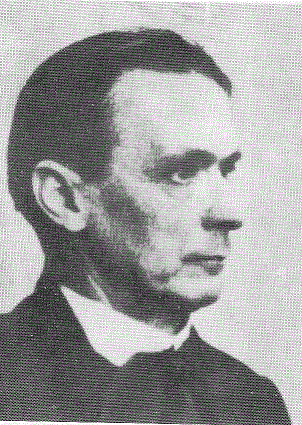
\includegraphics[scale=.4]{a20150217TheWayofLivingThought-img001.png}
\end{wrapfigure}

Among so many currents cited in the text, there is also Steiner's anthroposophy, to whom, however, Evola shows he was not particularly hostile, so much so that Guenon, after reading the text, reproached him for being too soft on the Austrian master. He recognized the value of the personality as well as the validity of specific methods that he proposed, which constitute nothing new, but heavily criticized Steiner's system for the contents referring to ``humanity", ``evolution", ``peace", etc., in fact, if taken literally, certain of Steiner's discourses can, to anyone who is accustomed to traditional language and ancient texts, appear as humanitarian and anti-traditional discourses, if not contextualized clearly. It seems difficult therefore to accept that Evola did not know that the whole had to be taken with a grain of salt and raises legitimate doubt that he had wanted to discourage more the adherence to anthroposophy as a ``sect", more than to the entire Steinerian discourse, understood as ``science of the spirit", as much to recognize the positivity of a scientific vocation to the supersensible, beyond romantic mysticism and religious devotion.

In fact, It is toward the end of the same passage, that Evola recognizes that the separation is possible and that the operative part of Steiner's Rosicrucian doctrine is valid and usable. Evola says of Steiner:

\begin{quotex}
In reality Steiner's activity was remarkable. He did not properly display the characteristics of a medium or a deranged man. Under certain aspects, on the contrary, one can say that one errs in the opposite direction, that is, of a scientific-systematic spirit at any cost. If many of his conceptions are not less fantastic than the theosophical, one can only say, unlike the latter, that in his madness there is much method. In his work we find the same incomprehension in regard to the law of karma, and transmigration reduced to reincarnation, the same evolutionistic superstitions, etc. Therefore, whoever is able to effect a type of purification of that view from historical temporality, could arrive at something valid. Is it possible to separate this minor part of the doctrine from the rest? That is not easy for a great number of the adherents. They swear by his magisterial word and woe to whoever touches even a single detail of the master's doctrine. On the other hand, it is very natural that at a certain level it becomes more convenient to set down carefully the visions of cosmic evolution and the rest, than to give oneself practically to the methods of individual initiation. But doctrinally the separation can be made, in the sense that one can recognize that Steiner gave some practical teachings and the criteria of discrimination that are valid, and that can be utilized with full independence from the rest: from evolution, from reincarnation, from Christ now working in us, from the ideals of mystical collectivity and the inevitable love and so on. He understands the fundamental point: it is necessary that man fully realizes the power of clear and distinct perception, of logical thinking, of objective vision. The ideal is an exact science of the supersensible. 

\end{quotex}

\hfill

\begin{quotex}
\textbf{Massimo Scaligero} was a personal friend to \textbf{Julius Evola}, who even introduced Scaligero to anthroposophy. Nevertheless, Scaligero had a broader spiritual perspective but is widely respected in most anthroposophical circles. Scaligero shared similar political opinions with Evola, writing for the same journals, and was likewise interested the spiritual roots of ancient Rome.

The rest of the article deals with the characteristics of an initiatic group. Unlike an exoteric tradition, which has an unbroken horizontal chain, an esoteric tradition comes vertically, from above. That is, it cannot be institutionalized and is recognized by its fruits as described.

Note: Scaligero's system is called ``living thought" or ``living thinking". 

\end{quotex}
\paragraph{Massimo Scaligero}
\begin{wrapfigure}{rt}{.3\textwidth}
	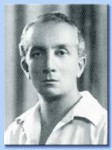
\includegraphics[scale=.7]{a20150217TheWayofLivingThought-img002.jpg}
\end{wrapfigure}
\textbf{Massimo Saligero}'s work has had a fundamental importance as the bridge between the world of anthroposophy, often challenged by the many ``deviations" that Evola mentioned, and Italian traditionalism in particular. He knew how to gather the ``operative" and ``realization" parts in Steiner's thought, leaving aside the social, pedagogical, and naturalistic parts. What counts for Scaligero is living thought, of which Steiner is the Master: the Master of the new age. He provided fundamental points to connect the ``science of the I", as outlined in the Ur and Krur volumes, to interior Work, to a ``preparation", an ``opus remotionis" to the Great Work. The path of Rosicrucianism and the Graal, the western and virile path par excellence, is undoubtedly linked to a double thread, to secret Hermetic and Wisdom paths that have run through the centuries since the Renaissance. Scaligero provides an interesting point of view on the relations between Evola and Steiner in \emph{From Yoga to Rosicrucianism}.



He is aware that the attacks against Steiner, which had to be expected from various fronts, not just from what was internal to anthroposophy itself, but especially by those who call themselves ``men of Tradition", including even Evola. The reason is simple: the ascesis of thought is a preliminary work of purification: it serves to make man sensitive to particular experiences that he can create on condition that he gains in the first place an inner balance and self-mastery, a mastery that must serve nowadays as the ``test" and thought, insofar as modern man is indubitably the ``cerebral" man. In the second place the gaining of an imaginative first dynamic is necessary, something whose necessity Evola did not perceive, through the fact of being in possession of such faculties through birth, through ``natural dignity", without this becoming the object of hard conquest, as is the case instead of common modern men, who try, perhaps titanically, to overcome and integrate human limits. From his point of view, Massimo Scaligero had a high opinion of Evola, as too many of his anthroposophical followers forget, who notoriously do not like our author who had altered the Master's doctrine (what a heresy!). It is in the text \emph{From Yoga to Rosicrucianism} that Scaligero speaks of his meeting with the Baron, who introduced him to Colazza thereby changing his life. Scaligero writes:

\begin{quotex}
With the passing of the years, I had to discover in him as the radiance value of the force that incarnated in a determinate nature, he had been able to subdue the very expression of knowledge to this. … on the way I understood about Evola that there could only be a single valid one of him and no copies: all of his teachings, yoga, tantrism, presuppose the original inner quality, the imaginative magic, that is a point of arrival for the modern seeker. In fact, Evola never had to be concerned about the conversion of reflexive thought, because he had no need of it, enjoying the use of thinking in movement like a congenial force to his personality: he was capable of conceiving liberation, but not his own autonomous movement as the beginning of the same liberation, insofar as identical with his own dialectic form. Evola's thinking spoke to me according to the world of forces to which he attached and this world of forces was important for me to realize, beyond the vision of things that his dialectic as personal expression belonged, just as beyond the dialectic value of Tradition to which he referred: value that for the evolians, not for Evola, is everything, and for which they find serious difficulties in realizing that world of forces. 

\end{quotex}
What to say of the synthesis? It is clear that Evola's work is fundamental for a worldview. Without it nothing would exist of the ``battle line of Tradition". Moreover, Evola did not provide a system except to indicate the methods of traditional realizations (yoga, Buddhism, Hermetism), but leaving imprecise the ``how" of achieving such experiences in a ``healthy" way. A propaedeutic preparation for that, in the opposite case, risks being transformed into a disastrous revival of the Promethean myth, if not in the experience of Ur, that as we said, includes multiple experiences of various initiatic schools. And here it gives way to the discourse of ``living thought" as purification, as preliminary ascesis, as the centration of itself and creation of a first intangible nucleus that can then confront the ``waters" without being overwhelmed by them.

\paragraph{Neo-Spiritualism and Tradition}
What then to say about those who, throwing out the baby with the bathwater (and the image seems to merit careful consideration), insert the entire representative of ``living thought" into the field of neo-spiritualism without thinking twice about it? The criticism that Evola brought previously in \emph{Mask and Face} is sound. The many esoteric schools, new religions, sects, and so on, that infest today's world are a clear proof. The litmus test of whatever esoteric, operative, or initiatic trend one wants to consider is to see if it leads to the strengthening of waking consciousness, or instead to the excitation of the emotive-irrational part of the disciple or even his actual animal nature. Even if it is not also a question of true deviations, at the edge of Satanism and the inversion of symbols and meanings, especially created by entities and forces in order to lead a man astray who still seeks from his real spiritual aspirations, then everything gets resolved in a devotionalism, in a religion of ``life", of the senses, and of ``freedom", meant in a pejorative sense.

All that is completely absent in the ``way of living thought" and in the Spiritual Science. It is indeed evident in Steiner's will to provide a ``solar way" that is averse to the subpersonal and to ``extrasensory" states, and that on the contrary tends to the development of the conscious individual, and not to a dissolution in a chaotic or naturalistic ``all". And this is the dry path, the solar path, the heroic and virile path par excellence. Hercules himself succumbed because he ``fell asleep" and made himself lose the result achieved with bitter struggle. Jacob wrestles with the angel of the Lord throughout the night: he remains awake and brings back victory. Gilgamesh loses his eternal youth he won by failing and falling prey to the symbolic ``sleep", that is, after all, the constant state of man's waking life, especially of modern man. The awakened man is, first of all, one who is present to himself, who lives in that which makes and marks himself and the meaning of every act of daily life. And this, it is granted, is very Roman and very Western.

It is just as obvious that the advocates of Tradition have overlooked a fundamental truth that Massimo Scaligero notes with masterful words: Tradition is a living force, not a crystallization of past experiences; it is not a worship of the past, nor sectarian dogmatism, nor a ``religion of esoterism". Instead it is a force that has taken, is taking, and will take the most various forms, able to lead the world to the Spirit, but that they are never the same, nor do they ever repeat themselves. Whoever thinks in a different way has understood nothing and confused the form with the substance. That fact that many ``traditionalists" persist in judging the work of Massimo Scaligero and of Rudolf Steiner through him, on the basis of hearsay, so it would be a matter of ``modern methods", not connected to any ``traditional regularity", is the index of a level of intellectual freedom and comprehension of a really low concept of ``spirituality".

For one simple reason: they judge the ``regularity" of a system, exposition, and doctrine not by what it transmits, by its living contents and by reaffirming eternal and immutable verities under apparent diversity and formulations, but by the fact that an author or a ``regular initiatic organization" has defined or at least appropriated it. Now, that the ascesis of thinking is not contained in the traditional texts of the most varied spiritualities is a natural question: the necessity of a similar ``Opus" was barely felt, at a minimum, only two or a thousand years ago, because a state that was natural for ``ancient" man is an object of conquest for ``modern" man. It is obvious that modern man is not easily comparable to the ancient Roman or to the Indian of the Vedas, and this will displease those who believe that the mere sentiment and admiration for an epoch will suffice in order to be like those who lived in that epoch.

But if the detractors of Scaligero, Steiner, Filippani Ronconi, and Colazza dared to study in depth the proposed practices, they would see that they differ very little, in substance, from what is the preparation for the Work in Hermetism, from the stoic presence in oneself, from many Platonic and Pythagorean practices and instructions. The fact that, in order to be considered traditionally regular, a supposed ``license" issued by a religion, sect, lodge, or group, is necessary with the contemporary desire to be attached to an ``uninterrupted chain" is the mantra that is raised against the way of living thought. That shows a subtle fear in them: the need for protection, or to be guided and led by the hand, something that is cloaked with the alleged ``respect for Tradition", when it is in reality the fear of acknowledging that the path of initiation has always been an individual journey and that, if in other periods there existed support represented by mysteriosophical religions and groups, now it is not the time of speak of it. We are convinced that initiatic organizations exist: but at a different level from what is commonly understood. It is not so much about groups of men, but rather of transcendent forces, that are waiting to welcome and guide those who will be made worthy. There is the Golden brotherhood of the Rose+Cross, awaiting disciples who will have achieved the polishing of the Stone.



\flrightit{Posted on 2015-02-17 by Aeneas }

\begin{center}* * *\end{center}

\begin{footnotesize}\begin{sffamily}



\texttt{Tom Blanchard on 2015-02-17 at 12:55 said: }

Interesting. What do you make of Tomberg, Levi, Agrippa, etc., who all were deeply involved in ceremonial/operative magic of this type, only to later dismiss it as a vanity (in Agrippa's case, specifically)? It is never denied that these operations are effective, but many of these authorities seem to indicate that their power is nevertheless insignificant compared to what can be achieved through ``standard" devotional mysticism. Although operative magic would seem for these men to have been at the very least a necessary stage through which they passed, they themselves insist to the contrary (again, thinking again of Agrippa in particular, who says that those who practice the arts he described when he was younger are destined to suffer the infernal fate of Simon Magus).


\hfill

\texttt{Scardanelli on 2015-02-17 at 15:00 said: }

Tom,

Did Tomberg involve himself in ceremonial magic? With his background it seems likely that he was active in the theurgy, but I would hesitate to identify theurgy with ceremonial magic. Tomberg does seem to equate the work of MArtinez de Pasqually with ceremonial magic at times, but it seems that Pasqually's methods are more in line with the sacred magic of the Empress or that described in Mouni Sadhu's work, Theurgy. 

Here is what Tomberg says about Agrippa:

\begin{quotationx}\scriptsize
Now, we occultists, magicians, esotericists and Hermeticists — all those who want to ``do" instead of merely waiting, who want ``to take their evolution in their own hands" and ``to direct it towards an aim"—are confronted with this choice in a much more dramatic way, I should say, than is so for people who are not concerned with esotericism. Our principal danger (if not the only true danger) is that of preferring the role of ``builders of the tower of Babel" (no matter whether personally or in a community) to watching over ``as gardeners or vine-growers the garden or the vine of the Lord". Truth to tell, the only truly morally founded reason for keeping esotericism ``esoteric", i.e. for not bringing it to the broad light of day and popularizing it, is the danger of the great misunderstanding of confusing the tower with the tree, as a consequence of which ``masons" will be recruited instead of ``gardeners".
…
And then the problem that disquieted Agrippa of Nettesheim, author of the classic work on magic, \textit{De Occulta Philosophia}: How could it be that the author of this book, in which one finds a multitude of things based on authentic experience, how could it be that he, the enthusiastic adept, became the skeptic disenchanted with life who wrote \textit{De Incertitudine et Vanitate Scientiarum} (``On the Uncertainty and the Vanity of the Sciences"), which was written during his last years of life? The answer to this question is that Agrippa had built a ``tower of Babel" which was later blasted by a ``thunderbolt from above". It was higher reality which made all the ``sciences of the supernatural" —to which he had devoted the best years of his life —appear vain to him. The tower was shaken, but the way of heaven was opened. He was free to begin again, i.e. in a condition to enter upon the way of growth.
\end{quotationx}

\hfill

\texttt{Jonathan Olavsson on 2015-02-17 at 15:49 said: }

Very interesting, Cologero. Thank you for translating and sharing this article, which certainly clarifies many of the questions about Evola's view on Steiner.

I have not read any of Steiner's works, but I know that most of it is translated into English, some of it even into the Scandinavian languages, of which Norwegian is my mother-tongue. Based on your own reading, Cologero, what would be the best place to start for an overview over some of the operative methods described by Steiner?


\hfill

\texttt{Cologero on 2015-02-17 at 21:55 said: }

Jonathan, I put a link to his Philosophy of Freedom, which is a good place to start. It predates his theosophical period. Perhaps then, there is Knowledge of the Higher World.

However, it may be more interesting to look at Massimo Scaligero's works, some of which have been translated into English. He tries to balance some (but not all) aspects of anthroposophy with Evolian style Tradition. Unfortunately, a few of his books seem to have been deliberately purged.


\hfill

\texttt{Cameron on 2015-02-18 at 16:39 said: }

Anthroposophists are not big on ceremonial magic, to my experience, unless you include the rites of the Christian Community church. Correct me if I'm wrong, but I'm assuming that the ``operative techniques" mentioned are referring to Steiner's extensive instructions for inner training, rather than anything ritualistic. A very interesting read, thank you.


\hfill

\texttt{Mark Citadel on 2015-02-18 at 23:33 said: }

To be honest, I had never even heard of Steiner, however if Evola gave him time it's worth looking into him.

Very interesting that Steiner had a supernatural, life-changing encounter with Christ that influenced his life. Reminds me of the reported encounter that Corneliu Codreanu had with the Archangel Michael, since of course he also had links to Evola.


\hfill

\texttt{Cologero on 2015-02-26 at 00:14 said: }

Mr. Citadel, Steiner is a frustrating blend of great insights and absurdities. Nevertheless, he has attracted some very intelligent men such as C S Lewis' friend Owen Barfield, Massimo Scaligero, and up to Valentin Tomberg. I'm not recommending going down that path.


\hfill

\texttt{David on 2015-02-23 at 01:10 said: }

Very interesting translation, thank you as always Cologero.


\hfill

\texttt{lee on 2015-02-23 at 04:14 said: }

Thank you for this translation Cologero. The section ``The litmus test of whatever esoteric, operative, or initiatic trend one wants to consider is to see if it leads to the strengthening of waking consciousness, or instead to the excitation of the emotive-irrational part of the disciple or even his actual animal nature" is so readily forgotten in my experience.


\hfill

\texttt{Scardanelli on 2015-02-23 at 10:39 said: }

Do you believe this purge was enacted by Anthroposophists? I've looked into Scaligero a bit and those surrounding him. I'm reading a book on meditation by Georg Kuhlewind ``The Light of the `I'", who was apparently a friend or student of Scalligero. In the preface he speaks about Scaligero and mentions that he agrees with his operative work, but disagrees on other points. Perhaps these ``other points" are Scaligero's ties with Evola and Traditionalism.

This is a rather interesting series. I appreciate the notion of initiation from above, and that initiation only becoming available when one has sufficiently purified himself through mental ascesis. This especially highlights the emptiness of the claims that the western initiation is no longer available. It is certainly available, but only to those who have made themselves worthy.


\hfill

\texttt{Cologero on 2015-02-25 at 23:38 said: }

Probably, Scardanelli. For some reason, there is a concerted effort to discredit the Waldorf schools, and Scaligero is a target. Seems like overkill for a rather obscure movement.


\hfill

\texttt{Max on 2016-01-30 at 06:53 said: }

A point that is emphasized by Scaligero is that Evola knew force, which becomes clear from reading his work, he was a ``shock treatment", awakening latent forces of the self. The pagan world knew forces and had names for them, but with Christ comes revelation of higher directing purpose, freeing us from the pagan conflict of various influences contending against each other. Scaligero seems to think that Evola did not follow his philosophy to its end, that he did not recognize the Logos, or what underlies the realization of the ``centrality and the invincibility of the I" in the universal order. The pagan mind with its many gods is like the equivalent of human personality, and even though one of them may be the ``chief god", this does not resolve things in a definite way. Evola had a strong personality, and was a ``powerful dialectician", not limited to a specific ideology or identity, whereas most people defend a point of view so viciously as if their life depended on it. To be consistent with Evola's ``path of action" one should probably pay more attention to what he does than what he says, being an ``evolian" makes no sense as there is no universal system to follow, and it seems like a negation of the very point he is trying to make, adhering to a ``science of the I". 

It is said that Tradition is a living force and as such one is either aligned with it or not. There is no middle ground and it can not be understood abstractly from a distance. When going from one place to another, the views along the road changes every moment even though the traveller and his intention do not change. Without an understanding of how one thing relates to another, for a passive observer, it merely looks like a collection of images with nothing in common.

There is a reference to the Rocicrucians, who are said to have left for the East. Considering they were purportedly an esoteric group, I am not sure it has to be read literally. Is not ``the east" somewhat like the end of the rainbow in that it always retreats further away when you attempt to go there? What is consistently ignored by most people is what is constant in every experience, they believe that neglecting who is actually experiencing something is the basis for objectivity, but this can not be true. Without ``someone there", there would not be any rainbow in the first place, since it manifests by observing it. One has to ask oneself who exactly it is that observes in modern science -an empty eye without body and without being, such as in the ``Lord of the Rings", incapable of either depth or colour?

Since there are always underlying assumptions, we can see by applying a small amount of common sense, for example to the perspective that ``the east" is the orient, that the point of reference or ``center" in this case must be Europe. By imagination however, man fantasizes about being in a different place than where he really is. This is a double edged sword: it allows us to conceive something which is not yet and thus make it come to pass, or it can pacify and restrict us to a simulated world of appearances with limited application to life. The good thing about willing and doing is that it reveals to us what was fantasy and what is not.


\end{sffamily}\end{footnotesize}
